\documentclass[fleqn,8pt]{latex/stylish_article} % Document font size and equations flushed left

\setcounter{tocdepth}{3}

% Pandoc environments
\usepackage{framed}
\usepackage{fancyvrb}
\providecommand{\tightlist}{%
  \setlength{\itemsep}{0pt}\setlength{\parskip}{0pt}}
\newcommand{\VerbBar}{|}
\newcommand{\VERB}{\Verb[commandchars=\\\{\}]}
\DefineVerbatimEnvironment{Highlighting}{Verbatim}{commandchars=\\\{\}, fontsize=\scriptsize} % R Code

% Colored code
\usepackage{color}
\definecolor{shadecolor}{RGB}{248,248,248}
\newenvironment{Shaded}{\begin{snugshade}}{\end{snugshade}}
\newcommand{\KeywordTok}[1]{\textcolor[rgb]{0.13,0.29,0.53}{\textbf{{#1}}}}
\newcommand{\DataTypeTok}[1]{\textcolor[rgb]{0.13,0.29,0.53}{{#1}}}
\newcommand{\DecValTok}[1]{\textcolor[rgb]{0.00,0.00,0.81}{{#1}}}
\newcommand{\BaseNTok}[1]{\textcolor[rgb]{0.00,0.00,0.81}{{#1}}}
\newcommand{\FloatTok}[1]{\textcolor[rgb]{0.00,0.00,0.81}{{#1}}}
\newcommand{\ConstantTok}[1]{\textcolor[rgb]{0.00,0.00,0.00}{{#1}}}
\newcommand{\CharTok}[1]{\textcolor[rgb]{0.31,0.60,0.02}{{#1}}}
\newcommand{\SpecialCharTok}[1]{\textcolor[rgb]{0.00,0.00,0.00}{{#1}}}
\newcommand{\StringTok}[1]{\textcolor[rgb]{0.31,0.60,0.02}{{#1}}}
\newcommand{\VerbatimStringTok}[1]{\textcolor[rgb]{0.31,0.60,0.02}{{#1}}}
\newcommand{\SpecialStringTok}[1]{\textcolor[rgb]{0.31,0.60,0.02}{{#1}}}
\newcommand{\ImportTok}[1]{{#1}}
\newcommand{\CommentTok}[1]{\textcolor[rgb]{0.56,0.35,0.01}{\textit{{#1}}}}
\newcommand{\DocumentationTok}[1]{\textcolor[rgb]{0.56,0.35,0.01}{\textbf{\textit{{#1}}}}}
\newcommand{\AnnotationTok}[1]{\textcolor[rgb]{0.56,0.35,0.01}{\textbf{\textit{{#1}}}}}
\newcommand{\CommentVarTok}[1]{\textcolor[rgb]{0.56,0.35,0.01}{\textbf{\textit{{#1}}}}}
\newcommand{\OtherTok}[1]{\textcolor[rgb]{0.56,0.35,0.01}{{#1}}}
\newcommand{\FunctionTok}[1]{\textcolor[rgb]{0.00,0.00,0.00}{{#1}}}
\newcommand{\VariableTok}[1]{\textcolor[rgb]{0.00,0.00,0.00}{{#1}}}
\newcommand{\ControlFlowTok}[1]{\textcolor[rgb]{0.13,0.29,0.53}{\textbf{{#1}}}}
\newcommand{\OperatorTok}[1]{\textcolor[rgb]{0.81,0.36,0.00}{\textbf{{#1}}}}
\newcommand{\BuiltInTok}[1]{{#1}}
\newcommand{\ExtensionTok}[1]{{#1}}
\newcommand{\PreprocessorTok}[1]{\textcolor[rgb]{0.56,0.35,0.01}{\textit{{#1}}}}
\newcommand{\AttributeTok}[1]{\textcolor[rgb]{0.77,0.63,0.00}{{#1}}}
\newcommand{\RegionMarkerTok}[1]{{#1}}
\newcommand{\InformationTok}[1]{\textcolor[rgb]{0.56,0.35,0.01}{\textbf{\textit{{#1}}}}}
\newcommand{\WarningTok}[1]{\textcolor[rgb]{0.56,0.35,0.01}{\textbf{\textit{{#1}}}}}
\newcommand{\AlertTok}[1]{\textcolor[rgb]{0.94,0.16,0.16}{{#1}}}
\newcommand{\ErrorTok}[1]{\textcolor[rgb]{0.64,0.00,0.00}{\textbf{{#1}}}}
\newcommand{\NormalTok}[1]{{#1}}

% cslreferences environment required by pandoc > 2.7

% Polyglossia
\usepackage{polyglossia}
\setmainlanguage{en-US}
\setotherlanguage{fr-FR}
\setotherlanguage{it}

% localized quotes
\usepackage[strict,autostyle]{csquotes}

% Figures
\usepackage{graphicx,grffile}
\makeatletter
\def\maxwidth{\ifdim\Gin@nat@width>\linewidth\linewidth\else\Gin@nat@width\fi}
\def\maxheight{\ifdim\Gin@nat@height>\textheight0.8\textheight\else\Gin@nat@height\fi}
\makeatother
% Scale images if necessary, so that they will not overflow the page
% margins by default, and it is still possible to overwrite the defaults
% using explicit options in \includegraphics[width, height, ...]{}
\setkeys{Gin}{width=\maxwidth,height=\maxheight,keepaspectratio}

% Additional packages
\usepackage{natbib}             % Advanced Bibliography (citep...).
\usepackage{amsmath,amsfonts,amssymb}
\usepackage{breqn}              % Line breaks in equations
\usepackage{url}                % Line breaks in url's
\usepackage{enumitem}           % Line spacing in lists
  \setlist[itemize]{noitemsep,nolistsep}
  \setlist[enumerate]{noitemsep,nolistsep}

% Tables
\usepackage{longtable,booktabs}
\usepackage{caption}
% These lines are needed to make table captions work with longtable:
\makeatletter
\def\fnum@table{\tablename~\thetable}
\makeatother
% longtable 2 columns
% https://tex.stackexchange.com/questions/161431/how-to-solve-longtable-is-not-in-1-column-mode-error
\makeatletter
\let\oldlt\longtable
\let\endoldlt\endlongtable
\def\longtable{\@ifnextchar[\longtable@i \longtable@ii}
\def\longtable@i[#1]{\begin{figure}[t]
\onecolumn
\begin{minipage}{0.5\textwidth}\scriptsize
\oldlt[#1]
}
\def\longtable@ii{\begin{figure}[t]
\onecolumn
\begin{minipage}{0.5\textwidth}\scriptsize
\oldlt
}
\def\endlongtable{\endoldlt
\end{minipage}
\twocolumn
\end{figure}}
\makeatother

% Full-width tables
\usepackage{tabu}
\renewenvironment{table}{\begin{table*}}{\end{table*}\ignorespacesafterend}

% Prevent overfull lines
\setlength{\emergencystretch}{3em}

% User-adder preamble
\hyphenation{quan-tile re-gres-sion out-li-ers het-ero-ske-das-tic}

% hyperref comes last
\usepackage{hyperref}           % Hypertext links, PDF bookmarks
  \hypersetup{%
    urlcolor=blue,%
    linkcolor=black,citecolor=black,colorlinks=true%
  }

%----------------------------------------------------------------------------------------
%	ARTICLE INFORMATION
%----------------------------------------------------------------------------------------

\JournalInfo{Working Paper, MSc in Statistics for Data Science, Carlos III University of Madrid} % Journal information
\Archive{DOI: N/A (internal report)} % Additional notes (e.g. copyright, DOI, review/research article)

\PaperTitle{Advance Regression Term Project} % Article title

\Authors{
Gerard Palomo \& Juan Pablo Uphoff\textsuperscript{}
} % Authors
\affiliation{

}
\affiliation{*\textbf{Corresponding author}: , \url{https://www.uc3m.es}} % Corresponding author

\Keywords{OLS, Quantile Regression, Machine Learning} % Keywords
\newcommand{\keywordname}{Keywords} % Defines the keywords heading name

\JEL{C45, C55} % JEL codes
\newcommand{\JELname}{JEL} % Defines the JEL heading name

\Acknowledgements{This report was completed for the course \textbf{Advanced Regression and Prediction}, as part of the \textbf{MSc in Statistics for Data Science} at \textbf{University Carlos III of Madrid}.} % Acknowledgements
\newcommand{\acknowledgementsname}{Acknowledgements} % Defines the heading name

%----------------------------------------------------------------------------------------
%	ABSTRACT
%----------------------------------------------------------------------------------------

\Abstract{
Linear quantile regression extends ordinary least squares (OLS) by modeling conditional quantiles of a response variable as linear functions of predictors. This offers a more complete view of the conditional distribution, revealing heterogeneous effects not captured by mean regression. Unlike OLS, quantile regression makes no strict distributional assumptions and is robust to outliers. We review the formulation, estimation, and inference for linear quantile regression, contrasting it with OLS. A simulation study compares OLS and quantile regression at various quantile levels (0.1 to 0.9) in both univariate and multivariate settings. We examine performance under normal and heavy-tailed error distributions, including scenarios with outliers, and assess the impact of sample size. The results illustrate that quantile regression estimates remain reliable under outlier contamination and uncover distributional effects (e.g.~heteroscedasticity) that OLS misses. All simulation code is provided in R for reproducibility.
}

%----------------------------------------------------------------------------------------

\begin{document}

\selectlanguage{en-US}

\flushbottom % Makes all text pages the same height

\maketitle % Print the title and abstract box

\tableofcontents % Print the contents section

\thispagestyle{empty} % Removes page numbering from the first page

%----------------------------------------------------------------------------------------
%	ARTICLE CONTENTS
%----------------------------------------------------------------------------------------

\section{Introduction.}\label{introduction.}

Regression analysis typically focuses on modeling the conditional mean of a response given predictors (as in ordinary least squares, OLS). In contrast, quantile regression (QR) aims to model conditional quantiles (e.g., median, quartiles) of the response variable. Koenker and Bassett (1978) first introduced linear quantile regression, generalizing the regression model beyond the mean to an ensemble of conditional quantile functions.

Quantile regression provides several advantages over OLS. First, it allows us to explore the entire conditional distribution of \(Y\) given \(X\), not just the mean, thereby revealing heterogeneous effects of predictors at different outcome levels . For example, an education variable might have a larger impact at the lower tail (10th percentile) of income than at the median or upper tail.

Second, quantile regression is robust to outliers in the response data. OLS estimates can be unduly influenced by a few extreme observations because it minimizes squared errors; in contrast, quantile regression (especially median regression) uses absolute-error-based loss, making it less sensitive to extreme \(Y\) values.

Third, quantile methods remain valid under skewed or heteroskedastic distributions. OLS relies on homoscedasticity and normality assumptions for optimality and inference, whereas quantile regression imposes no such requirements and can capture distributional changes (e.g., increasing variance) across predictor levels.

There are, of course, other approaches to address OLS limitations. Notably, researchers have developed robust regression methods and penalization techniques. For instance, Fan and Li (2001) proposed nonconcave penalized likelihood methods for variable selection, which can be applied to robust regression models.

In this article, we provide an overview of linear quantile regression theory (Section 2) and present a simulation study (Section 3) comparing quantile regression to OLS under various scenarios. We consider both univariate and multivariate predictor cases, examine performance at multiple quantile levels, and evaluate robustness to outliers and sample size changes. A concluding section summarizes the findings. Throughout, we cite key references, including Koenker and Hallock (2001) for an accessible overview, and Fan and Li (2001) for context on related regression advances. The complete R code for our analysis is provided in the Appendix to ensure reproducibility.

\section{2. Linear Quantile Regression: Theory and Methods}\label{linear-quantile-regression-theory-and-methods}

\subsection{Definition and Estimation}\label{definition-and-estimation}

For a random variable \(Y\), the \(\tau\)-th quantile is the value \(q_\tau\) such that \(P(Y \le q_\tau) = \tau\). In a regression setting, \textbf{quantile regression (QR)} estimates:

\[
Q_Y(\tau \mid X = x) = x^\top \beta(\tau),
\]

where \(\beta(\tau)\) is a vector of coefficients specific to quantile level \(\tau\). For example, \(\beta_1(0.5)\) represents the effect of \(X_1\) on the median of \(Y\).

Koenker and Bassett (1978) proposed estimating \(\beta(\tau)\) by minimizing the \textbf{check loss}:

\[
\hat\beta(\tau) = \arg\min_\beta \sum_{i=1}^n \rho_\tau(y_i - x_i^\top \beta),
\]

with \(\rho_\tau(u) = u(\tau - \mathbb{I}\{u < 0\})\). For \(\tau = 0.5\), this reduces to \textbf{least absolute deviations (LAD)} regression.

Each \(\tau\) is estimated independently using linear programming, and the family \(\{\beta(\tau)\}\) forms a \textbf{quantile process} describing the full conditional distribution of \(Y\).

\subsection{Inference}\label{inference}

Under regularity conditions, \(\hat\beta(\tau)\) is asymptotically normal:

\[
\sqrt{n}(\hat\beta(\tau) - \beta(\tau)) \overset{d}{\to} N(0, \Sigma(\tau)),
\]

with variance estimators obtained via \textbf{bootstrapping} or \textbf{sandwich estimators} (Koenker, 2005). Practical inference is available via \texttt{summary()} in the R package \texttt{quantreg}.

\subsection{Comparison to OLS}\label{comparison-to-ols}

OLS estimates the conditional mean:

\[
\mathbb{E}[Y \mid X = x] = x^\top \beta,
\]

whereas QR estimates conditional quantiles. When errors are symmetric and homoscedastic, QR and OLS give similar results. Otherwise, QR captures \textbf{distributional heterogeneity}, such as increasing variance or skewness.

Moreover, QR is \textbf{robust to outliers in \(Y\)}, unlike OLS which minimizes squared error and is sensitive to extreme values. QR also allows different slopes across quantiles, offering richer interpretation.

In the next section, we illustrate these theoretical advantages through a simulation study.

\section{3. Simulation Study}\label{simulation-study}

This section presents a Monte Carlo simulation study designed to compare the performance of \textbf{Ordinary Least Squares (OLS)} and \textbf{Quantile Regression (QR)} estimators under controlled, interpretable scenarios. Our aim is to assess how both methods behave across different quantiles of the conditional distribution, particularly under heteroskedasticity, outlier contamination, and varying sample sizes.

\subsection{3.1 Data Generating Process (DGP)}\label{data-generating-process-dgp}

We consider the linear model:

\[
Y = \beta_0 + \beta_1 X_1 + \beta_2 X_2 + \varepsilon,
\]

with fixed parameters \(\beta_0 = 5\), \(\beta_1 = 1.5\), and \(\beta_2 = -1\). In the univariate setting, only \(X_1\) is included; in the multivariate setting, both \(X_1\) and \(X_2\) are active predictors.

\begin{itemize}
\tightlist
\item
  \textbf{Covariates}: \(X_1, X_2 \overset{iid}{\sim} \text{Uniform}(0,10)\).
\item
  \textbf{Error term} \(\varepsilon\) follows different structures to emulate classical and adversarial settings (see below).
\item
  \textbf{Quantiles studied}: \(\tau = 0.1\), \(0.5\), \(0.9\) to represent lower, central, and upper tails of the conditional distribution.
\end{itemize}

We focus on:
- \textbf{Small to large sample regimes}: \(n = 50\), \(100\), \(200\), and \(1000\).
- \textbf{Replications}: Each configuration is simulated over 100 independent datasets to stabilize the evaluation of finite-sample properties.

The sample sizes were chosen to explore both low-\(n\) variability and convergence behavior, with \(n=100\) serving as a baseline and \(n=1000\) approximating asymptotic regimes.

We estimate parameters using:
- \texttt{lm()} for OLS (minimizing squared loss)
- \texttt{rq()} from the \texttt{quantreg} package for QR at various \(\tau\) values (minimizing asymmetric absolute loss; see Section 2).

\subsection{3.2 Simulation Setup}\label{simulation-setup}

We evaluate the estimators under three error structures:

\begin{itemize}
\item
  \textbf{Homoscedastic Gaussian}:
  \(\varepsilon_i \sim \mathcal{N}(0, \sigma^2),\ \sigma=2\). This setting satisfies OLS assumptions and serves as a benchmark.
\item
  \textbf{Contaminated Gaussian (outliers)}:
  \(\varepsilon_i = Z_i + O_i\) with \(Z_i \sim \mathcal{N}(0,2^2)\) and \(O_i = 30\) with probability \(p = 0.05\). This mimics a heavy-tailed distribution or a mixture contamination model, testing robustness. Outliers are introduced:

  \begin{itemize}
  \tightlist
  \item
    randomly (to simulate noise in \(Y\)),
  \item
    or conditionally (e.g.~to the largest \(X_1\)) to induce high-leverage effects.
  \end{itemize}
\item
  \textbf{Heteroskedastic}:
  \(\varepsilon_i \sim \mathcal{N}(0,\sigma^2(X_i))\) with \(\sigma(X_i) = 1 + 0.2 X_1\). This setting creates increasing spread in \(Y\) conditional on \(X_1\), violating OLS homoscedasticity.
\end{itemize}

\subsection{3.3 Evaluation Metrics}\label{evaluation-metrics}

For each simulation, we extract the slope estimates (primarily for \(\beta_1\)) and compute:

\begin{itemize}
\item
  \textbf{Bias}:
  \[ 
  \text{Bias}(\hat\beta) = \mathbb{E}[\hat\beta] - \beta
  \]
\item
  \textbf{RMSE}:
  \[
  \text{RMSE}(\hat\beta) = \sqrt{\mathbb{E}[(\hat\beta - \beta)^2]}
  \]
\item
  \textbf{Empirical variability}: Standard deviation of estimates across replications.
\end{itemize}

Along with some graphical support, these evaluations provide insight into estimator consistency, robustness, and efficiency under both ideal and adversarial conditions.

The theoretical basis for QR (Section 2) suggests that:
- OLS is optimal under homoscedastic Gaussian errors (Gauss-Markov assumptions),
- QR provides robust, distribution-sensitive estimation that remains valid when these assumptions are violated.

This simulation seeks to verify those expectations empirically.

\subsection{3.4 Simulation}\label{simulation}

\begin{Shaded}
\begin{Highlighting}[]
\FunctionTok{library}\NormalTok{(gridExtra)}
\NormalTok{plot\_one }\OtherTok{\textless{}{-}} \ControlFlowTok{function}\NormalTok{(data, model, title) \{}
    \FunctionTok{ggplot}\NormalTok{(data, }\FunctionTok{aes}\NormalTok{(}\AttributeTok{x =}\NormalTok{ x1, }\AttributeTok{y =}\NormalTok{ y)) }\SpecialCharTok{+} \FunctionTok{geom\_point}\NormalTok{(}\AttributeTok{alpha =} \FloatTok{0.5}\NormalTok{) }\SpecialCharTok{+}
        \FunctionTok{geom\_smooth}\NormalTok{(}\AttributeTok{method =} \StringTok{"lm"}\NormalTok{, }\AttributeTok{se =} \ConstantTok{FALSE}\NormalTok{, }\AttributeTok{color =} \StringTok{"red"}\NormalTok{,}
            \AttributeTok{linetype =} \StringTok{"dashed"}\NormalTok{) }\SpecialCharTok{+} \FunctionTok{geom\_quantile}\NormalTok{(}\AttributeTok{quantiles =}\NormalTok{ tau\_levels,}
        \AttributeTok{color =} \StringTok{"blue"}\NormalTok{, }\AttributeTok{size =} \FloatTok{0.8}\NormalTok{) }\SpecialCharTok{+} \FunctionTok{ggtitle}\NormalTok{(title) }\SpecialCharTok{+}
        \FunctionTok{theme\_minimal}\NormalTok{()}
\NormalTok{\}}
\FunctionTok{grid.arrange}\NormalTok{(}\FunctionTok{plot\_one}\NormalTok{(scenarios}\SpecialCharTok{$}\NormalTok{clean\_uni, models}\SpecialCharTok{$}\NormalTok{clean\_uni,}
    \StringTok{"Clean Univariate"}\NormalTok{), }\FunctionTok{plot\_one}\NormalTok{(scenarios}\SpecialCharTok{$}\NormalTok{outlier\_uni,}
\NormalTok{    models}\SpecialCharTok{$}\NormalTok{outlier\_uni, }\StringTok{"Outlier Univariate"}\NormalTok{), }\FunctionTok{plot\_one}\NormalTok{(scenarios}\SpecialCharTok{$}\NormalTok{clean\_multi,}
\NormalTok{    models}\SpecialCharTok{$}\NormalTok{clean\_multi, }\StringTok{"Clean Multivariate"}\NormalTok{), }\FunctionTok{plot\_one}\NormalTok{(scenarios}\SpecialCharTok{$}\NormalTok{outlier\_multi,}
\NormalTok{    models}\SpecialCharTok{$}\NormalTok{outlier\_multi, }\StringTok{"Outlier Multivariate"}\NormalTok{),}
    \AttributeTok{ncol =} \DecValTok{2}\NormalTok{)}
\end{Highlighting}
\end{Shaded}

\begin{figure}

{\centering 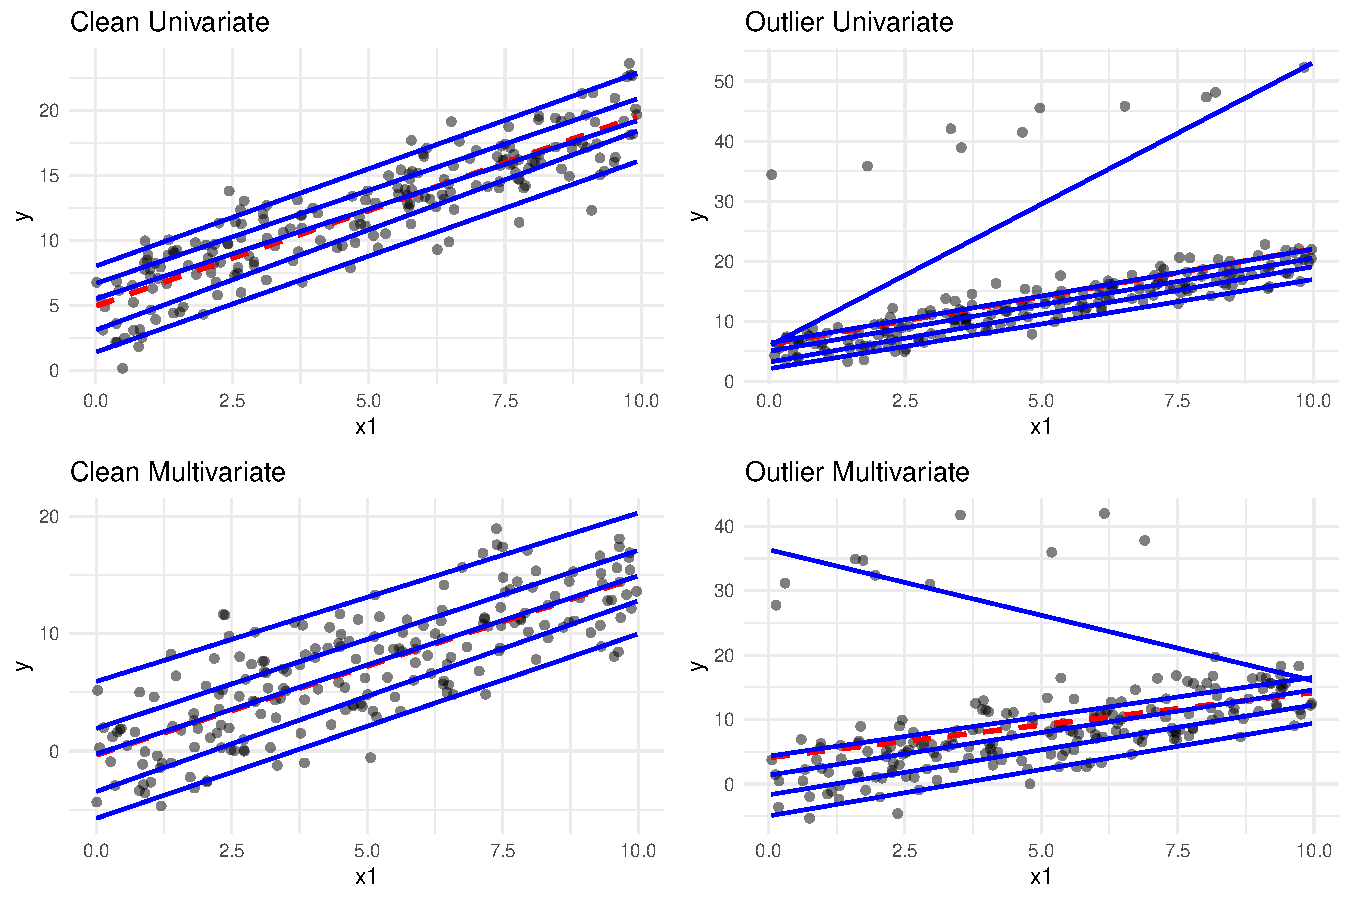
\includegraphics[width=0.8\linewidth]{ADR_project_files/figure-latex/boxplots-2x2-1} 

}

\caption{Comparison of slope estimates across settings}\label{fig:boxplots-2x2}
\end{figure}

\begin{Shaded}
\begin{Highlighting}[]
\NormalTok{summarize\_slopes }\OtherTok{\textless{}{-}} \ControlFlowTok{function}\NormalTok{(model) \{}
\NormalTok{    slopes }\OtherTok{\textless{}{-}} \FunctionTok{sapply}\NormalTok{(model}\SpecialCharTok{$}\NormalTok{qrs, }\ControlFlowTok{function}\NormalTok{(m) }\FunctionTok{coef}\NormalTok{(m)[}\StringTok{"x1"}\NormalTok{])}
    \FunctionTok{tibble}\NormalTok{(}\AttributeTok{Method =} \FunctionTok{c}\NormalTok{(}\FunctionTok{paste0}\NormalTok{(}\StringTok{"QR (tau="}\NormalTok{, tau\_levels,}
        \StringTok{")"}\NormalTok{), }\StringTok{"OLS"}\NormalTok{), }\AttributeTok{Estimate =} \FunctionTok{c}\NormalTok{(slopes, }\FunctionTok{coef}\NormalTok{(model}\SpecialCharTok{$}\NormalTok{ols)[}\StringTok{"x1"}\NormalTok{]))}
\NormalTok{\}}
\FunctionTok{summarize\_slopes}\NormalTok{(models}\SpecialCharTok{$}\NormalTok{clean\_uni)}
\end{Highlighting}
\end{Shaded}

\section{A tibble: 6 x 2}\label{a-tibble-6-x-2}

Method Estimate
1 QR (tau=0.05) 1.48
2 QR (tau=0.25) 1.54
3 QR (tau=0.5) 1.38
4 QR (tau=0.75) 1.43
5 QR (tau=0.95) 1.50
6 OLS 1.47

\begin{Shaded}
\begin{Highlighting}[]
\FunctionTok{set.seed}\NormalTok{(}\DecValTok{666}\NormalTok{)}
\NormalTok{data\_heterosk }\OtherTok{\textless{}{-}} \FunctionTok{simulate\_data}\NormalTok{(}\AttributeTok{n =} \DecValTok{1000}\NormalTok{, }\AttributeTok{heterosk =} \ConstantTok{TRUE}\NormalTok{)}
\NormalTok{fits\_heterosk }\OtherTok{\textless{}{-}} \FunctionTok{lapply}\NormalTok{(}\FunctionTok{seq}\NormalTok{(}\FloatTok{0.05}\NormalTok{, }\FloatTok{0.95}\NormalTok{, }\FloatTok{0.05}\NormalTok{), }\ControlFlowTok{function}\NormalTok{(tau) }\FunctionTok{rq}\NormalTok{(y }\SpecialCharTok{\textasciitilde{}}
\NormalTok{    x1, }\AttributeTok{tau =}\NormalTok{ tau, }\AttributeTok{data =}\NormalTok{ data\_heterosk))}
\NormalTok{slopes\_heterosk }\OtherTok{\textless{}{-}} \FunctionTok{sapply}\NormalTok{(fits\_heterosk, }\ControlFlowTok{function}\NormalTok{(fit) }\FunctionTok{coef}\NormalTok{(fit)[}\DecValTok{2}\NormalTok{])}
\NormalTok{ols\_slope }\OtherTok{\textless{}{-}} \FunctionTok{coef}\NormalTok{(}\FunctionTok{lm}\NormalTok{(y }\SpecialCharTok{\textasciitilde{}}\NormalTok{ x1, }\AttributeTok{data =}\NormalTok{ data\_heterosk))[}\DecValTok{2}\NormalTok{]}
\NormalTok{plot\_df }\OtherTok{\textless{}{-}} \FunctionTok{tibble}\NormalTok{(}\AttributeTok{tau =} \FunctionTok{seq}\NormalTok{(}\FloatTok{0.05}\NormalTok{, }\FloatTok{0.95}\NormalTok{, }\FloatTok{0.05}\NormalTok{), }\AttributeTok{slope =}\NormalTok{ slopes\_heterosk)}
\FunctionTok{ggplot}\NormalTok{(plot\_df, }\FunctionTok{aes}\NormalTok{(}\AttributeTok{x =}\NormalTok{ tau, }\AttributeTok{y =}\NormalTok{ slope)) }\SpecialCharTok{+} \FunctionTok{geom\_line}\NormalTok{(}\AttributeTok{color =} \StringTok{"blue"}\NormalTok{) }\SpecialCharTok{+}
    \FunctionTok{geom\_point}\NormalTok{(}\AttributeTok{color =} \StringTok{"blue"}\NormalTok{) }\SpecialCharTok{+} \FunctionTok{geom\_hline}\NormalTok{(}\AttributeTok{yintercept =}\NormalTok{ ols\_slope,}
    \AttributeTok{color =} \StringTok{"red"}\NormalTok{, }\AttributeTok{linetype =} \StringTok{"dashed"}\NormalTok{) }\SpecialCharTok{+} \FunctionTok{labs}\NormalTok{(}\AttributeTok{x =} \StringTok{"Quantile (tau)"}\NormalTok{,}
    \AttributeTok{y =} \StringTok{"Slope"}\NormalTok{, }\AttributeTok{title =} \StringTok{"Slope vs Quantile Level"}\NormalTok{) }\SpecialCharTok{+}
    \FunctionTok{theme\_minimal}\NormalTok{()}
\end{Highlighting}
\end{Shaded}

\begin{figure}

{\centering 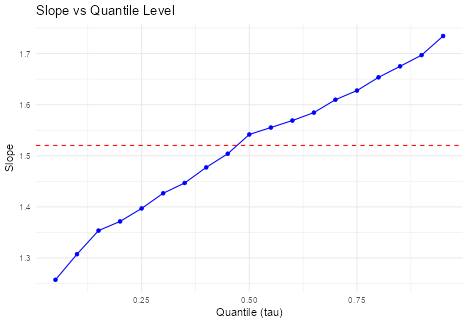
\includegraphics[width=0.8\linewidth]{ADR_project_files/figure-latex/plot-coef-vs-quantile-1} 

}

\caption{Slope vs Quantile for heteroskedastic case}\label{fig:plot-coef-vs-quantile}
\end{figure}

\begin{Shaded}
\begin{Highlighting}[]
\NormalTok{fit25 }\OtherTok{\textless{}{-}} \FunctionTok{rq}\NormalTok{(y }\SpecialCharTok{\textasciitilde{}}\NormalTok{ x1, }\AttributeTok{tau =} \FloatTok{0.25}\NormalTok{, }\AttributeTok{data =}\NormalTok{ scenarios}\SpecialCharTok{$}\NormalTok{clean\_uni)}
\NormalTok{fit50 }\OtherTok{\textless{}{-}} \FunctionTok{rq}\NormalTok{(y }\SpecialCharTok{\textasciitilde{}}\NormalTok{ x1, }\AttributeTok{tau =} \FloatTok{0.5}\NormalTok{, }\AttributeTok{data =}\NormalTok{ scenarios}\SpecialCharTok{$}\NormalTok{clean\_uni)}
\NormalTok{fit75 }\OtherTok{\textless{}{-}} \FunctionTok{rq}\NormalTok{(y }\SpecialCharTok{\textasciitilde{}}\NormalTok{ x1, }\AttributeTok{tau =} \FloatTok{0.75}\NormalTok{, }\AttributeTok{data =}\NormalTok{ scenarios}\SpecialCharTok{$}\NormalTok{clean\_uni)}
\FunctionTok{anova}\NormalTok{(fit25, fit50, fit75)}
\end{Highlighting}
\end{Shaded}

\begin{verbatim}
## Quantile Regression Analysis of Deviance Table
## 
## Model: y ~ x1
## Joint Test of Equality of Slopes: tau in {  0.25 0.5 0.75  }
## 
##   Df Resid Df F value  Pr(>F)  
## 1  2      598  2.9672 0.05221 .
## ---
## Signif. codes:  
## 0 '***' 0.001 '**' 0.01 '*' 0.05 '.' 0.1 ' ' 1
\end{verbatim}

\begin{Shaded}
\begin{Highlighting}[]
\CommentTok{\# kbl(anova\_table, caption = \textquotesingle{}Joint Test of}
\CommentTok{\# Equality of Slopes at Different Quantiles\textquotesingle{}) \%\textgreater{}\%}
\CommentTok{\# kable\_styling(latex\_options = \textquotesingle{}striped\textquotesingle{})}
\end{Highlighting}
\end{Shaded}

\begin{Shaded}
\begin{Highlighting}[]
\FunctionTok{library}\NormalTok{(quantreg)}
\FunctionTok{library}\NormalTok{(gridExtra)}
\FunctionTok{library}\NormalTok{(dplyr)}
\CommentTok{\# Simulate basic heteroskedastic data}
\FunctionTok{set.seed}\NormalTok{(}\DecValTok{666}\NormalTok{)}
\NormalTok{n }\OtherTok{\textless{}{-}} \DecValTok{500}
\NormalTok{X }\OtherTok{\textless{}{-}} \FunctionTok{runif}\NormalTok{(n, }\DecValTok{0}\NormalTok{, }\DecValTok{10}\NormalTok{)}
\NormalTok{epsilon }\OtherTok{\textless{}{-}} \FunctionTok{rnorm}\NormalTok{(n, }\AttributeTok{mean =} \DecValTok{0}\NormalTok{, }\AttributeTok{sd =} \DecValTok{1} \SpecialCharTok{+} \FloatTok{0.3} \SpecialCharTok{*}\NormalTok{ X)}
\NormalTok{Y }\OtherTok{\textless{}{-}} \DecValTok{5} \SpecialCharTok{+} \FloatTok{1.5} \SpecialCharTok{*}\NormalTok{ X }\SpecialCharTok{+}\NormalTok{ epsilon}
\NormalTok{data }\OtherTok{\textless{}{-}} \FunctionTok{data.frame}\NormalTok{(}\AttributeTok{X =}\NormalTok{ X, }\AttributeTok{Y =}\NormalTok{ Y)}
\CommentTok{\# Fit models}
\NormalTok{ols\_fit }\OtherTok{\textless{}{-}} \FunctionTok{lm}\NormalTok{(Y }\SpecialCharTok{\textasciitilde{}}\NormalTok{ X, }\AttributeTok{data =}\NormalTok{ data)}
\NormalTok{rq\_10 }\OtherTok{\textless{}{-}} \FunctionTok{rq}\NormalTok{(Y }\SpecialCharTok{\textasciitilde{}}\NormalTok{ X, }\AttributeTok{tau =} \FloatTok{0.1}\NormalTok{, }\AttributeTok{data =}\NormalTok{ data)}
\NormalTok{rq\_50 }\OtherTok{\textless{}{-}} \FunctionTok{rq}\NormalTok{(Y }\SpecialCharTok{\textasciitilde{}}\NormalTok{ X, }\AttributeTok{tau =} \FloatTok{0.5}\NormalTok{, }\AttributeTok{data =}\NormalTok{ data)}
\NormalTok{rq\_90 }\OtherTok{\textless{}{-}} \FunctionTok{rq}\NormalTok{(Y }\SpecialCharTok{\textasciitilde{}}\NormalTok{ X, }\AttributeTok{tau =} \FloatTok{0.9}\NormalTok{, }\AttributeTok{data =}\NormalTok{ data)}
\CommentTok{\# Plot 1: Scatterplot + regression lines}
\NormalTok{p1 }\OtherTok{\textless{}{-}} \FunctionTok{ggplot}\NormalTok{(data, }\FunctionTok{aes}\NormalTok{(}\AttributeTok{x =}\NormalTok{ X, }\AttributeTok{y =}\NormalTok{ Y)) }\SpecialCharTok{+} \FunctionTok{geom\_point}\NormalTok{(}\AttributeTok{alpha =} \FloatTok{0.4}\NormalTok{) }\SpecialCharTok{+}
    \FunctionTok{geom\_smooth}\NormalTok{(}\AttributeTok{method =} \StringTok{"lm"}\NormalTok{, }\AttributeTok{se =} \ConstantTok{FALSE}\NormalTok{, }\AttributeTok{color =} \StringTok{"red"}\NormalTok{,}
        \AttributeTok{linetype =} \StringTok{"dashed"}\NormalTok{) }\SpecialCharTok{+} \FunctionTok{geom\_quantile}\NormalTok{(}\AttributeTok{quantiles =} \FunctionTok{c}\NormalTok{(}\FloatTok{0.1}\NormalTok{,}
    \FloatTok{0.5}\NormalTok{, }\FloatTok{0.9}\NormalTok{), }\AttributeTok{color =} \StringTok{"blue"}\NormalTok{, }\AttributeTok{size =} \FloatTok{0.8}\NormalTok{) }\SpecialCharTok{+} \FunctionTok{labs}\NormalTok{(}\AttributeTok{title =} \StringTok{"OLS vs Quantile Regression Lines"}\NormalTok{,}
    \AttributeTok{y =} \StringTok{"Y"}\NormalTok{, }\AttributeTok{x =} \StringTok{"X"}\NormalTok{) }\SpecialCharTok{+} \FunctionTok{theme\_minimal}\NormalTok{()}
\CommentTok{\# Plot 2: Slope across quantiles}
\NormalTok{taus }\OtherTok{\textless{}{-}} \FunctionTok{seq}\NormalTok{(}\FloatTok{0.05}\NormalTok{, }\FloatTok{0.95}\NormalTok{, }\AttributeTok{by =} \FloatTok{0.05}\NormalTok{)}
\NormalTok{slopes }\OtherTok{\textless{}{-}} \FunctionTok{sapply}\NormalTok{(taus, }\ControlFlowTok{function}\NormalTok{(tau) }\FunctionTok{coef}\NormalTok{(}\FunctionTok{rq}\NormalTok{(Y }\SpecialCharTok{\textasciitilde{}}\NormalTok{ X,}
    \AttributeTok{tau =}\NormalTok{ tau))[}\DecValTok{2}\NormalTok{])}
\NormalTok{p2 }\OtherTok{\textless{}{-}} \FunctionTok{ggplot}\NormalTok{(}\FunctionTok{data.frame}\NormalTok{(}\AttributeTok{tau =}\NormalTok{ taus, }\AttributeTok{slope =}\NormalTok{ slopes),}
    \FunctionTok{aes}\NormalTok{(}\AttributeTok{x =}\NormalTok{ tau, }\AttributeTok{y =}\NormalTok{ slope)) }\SpecialCharTok{+} \FunctionTok{geom\_line}\NormalTok{(}\AttributeTok{color =} \StringTok{"blue"}\NormalTok{) }\SpecialCharTok{+}
    \FunctionTok{geom\_hline}\NormalTok{(}\AttributeTok{yintercept =} \FunctionTok{coef}\NormalTok{(ols\_fit)[}\DecValTok{2}\NormalTok{], }\AttributeTok{linetype =} \StringTok{"dashed"}\NormalTok{,}
        \AttributeTok{color =} \StringTok{"red"}\NormalTok{) }\SpecialCharTok{+} \FunctionTok{labs}\NormalTok{(}\AttributeTok{title =} \StringTok{"Slope estimates across quantiles"}\NormalTok{,}
    \AttributeTok{y =} \StringTok{"Slope"}\NormalTok{, }\AttributeTok{x =} \StringTok{"Quantile (tau)"}\NormalTok{) }\SpecialCharTok{+} \FunctionTok{theme\_minimal}\NormalTok{()}
\CommentTok{\# Plot 3: Robustness to outliers}
\NormalTok{data\_outlier }\OtherTok{\textless{}{-}}\NormalTok{ data}
\NormalTok{idx }\OtherTok{\textless{}{-}} \FunctionTok{sample}\NormalTok{(}\DecValTok{1}\SpecialCharTok{:}\NormalTok{n, }\DecValTok{10}\NormalTok{)}
\NormalTok{data\_outlier}\SpecialCharTok{$}\NormalTok{Y[idx] }\OtherTok{\textless{}{-}}\NormalTok{ data\_outlier}\SpecialCharTok{$}\NormalTok{Y[idx] }\SpecialCharTok{+} \DecValTok{50}  \CommentTok{\# Add strong outliers}
\NormalTok{ols\_fit\_outlier }\OtherTok{\textless{}{-}} \FunctionTok{lm}\NormalTok{(Y }\SpecialCharTok{\textasciitilde{}}\NormalTok{ X, }\AttributeTok{data =}\NormalTok{ data\_outlier)}
\NormalTok{rq\_50\_outlier }\OtherTok{\textless{}{-}} \FunctionTok{rq}\NormalTok{(Y }\SpecialCharTok{\textasciitilde{}}\NormalTok{ X, }\AttributeTok{tau =} \FloatTok{0.5}\NormalTok{, }\AttributeTok{data =}\NormalTok{ data\_outlier)}
\NormalTok{p3 }\OtherTok{\textless{}{-}} \FunctionTok{ggplot}\NormalTok{(data\_outlier, }\FunctionTok{aes}\NormalTok{(}\AttributeTok{x =}\NormalTok{ X, }\AttributeTok{y =}\NormalTok{ Y)) }\SpecialCharTok{+} \FunctionTok{geom\_point}\NormalTok{(}\AttributeTok{alpha =} \FloatTok{0.4}\NormalTok{) }\SpecialCharTok{+}
    \FunctionTok{geom\_smooth}\NormalTok{(}\AttributeTok{method =} \StringTok{"lm"}\NormalTok{, }\AttributeTok{se =} \ConstantTok{FALSE}\NormalTok{, }\AttributeTok{color =} \StringTok{"red"}\NormalTok{,}
        \AttributeTok{linetype =} \StringTok{"dashed"}\NormalTok{) }\SpecialCharTok{+} \FunctionTok{geom\_abline}\NormalTok{(}\AttributeTok{intercept =} \FunctionTok{coef}\NormalTok{(rq\_50\_outlier)[}\DecValTok{1}\NormalTok{],}
    \AttributeTok{slope =} \FunctionTok{coef}\NormalTok{(rq\_50\_outlier)[}\DecValTok{2}\NormalTok{], }\AttributeTok{color =} \StringTok{"blue"}\NormalTok{) }\SpecialCharTok{+}
    \FunctionTok{labs}\NormalTok{(}\AttributeTok{title =} \StringTok{"Effect of Outliers: OLS vs Median QR"}\NormalTok{,}
        \AttributeTok{y =} \StringTok{"Y"}\NormalTok{, }\AttributeTok{x =} \StringTok{"X"}\NormalTok{) }\SpecialCharTok{+} \FunctionTok{theme\_minimal}\NormalTok{()}
\CommentTok{\# Plot 4: Residuals histograms}
\NormalTok{residuals\_ols }\OtherTok{\textless{}{-}} \FunctionTok{resid}\NormalTok{(ols\_fit)}
\NormalTok{residuals\_rq50 }\OtherTok{\textless{}{-}} \FunctionTok{resid}\NormalTok{(rq\_50)}
\NormalTok{residuals\_df }\OtherTok{\textless{}{-}} \FunctionTok{data.frame}\NormalTok{(}\AttributeTok{residuals =} \FunctionTok{c}\NormalTok{(residuals\_ols,}
\NormalTok{    residuals\_rq50), }\AttributeTok{Method =} \FunctionTok{rep}\NormalTok{(}\FunctionTok{c}\NormalTok{(}\StringTok{"OLS"}\NormalTok{, }\StringTok{"QR (tau=0.5)"}\NormalTok{),}
    \AttributeTok{each =}\NormalTok{ n))}
\NormalTok{p4 }\OtherTok{\textless{}{-}} \FunctionTok{ggplot}\NormalTok{(residuals\_df, }\FunctionTok{aes}\NormalTok{(}\AttributeTok{x =}\NormalTok{ residuals, }\AttributeTok{fill =}\NormalTok{ Method)) }\SpecialCharTok{+}
    \FunctionTok{geom\_histogram}\NormalTok{(}\AttributeTok{alpha =} \FloatTok{0.5}\NormalTok{, }\AttributeTok{position =} \StringTok{"identity"}\NormalTok{,}
        \AttributeTok{bins =} \DecValTok{30}\NormalTok{) }\SpecialCharTok{+} \FunctionTok{facet\_wrap}\NormalTok{(}\SpecialCharTok{\textasciitilde{}}\NormalTok{Method) }\SpecialCharTok{+} \FunctionTok{labs}\NormalTok{(}\AttributeTok{title =} \StringTok{"Residuals Distribution: OLS vs QR"}\NormalTok{,}
    \AttributeTok{x =} \StringTok{"Residuals"}\NormalTok{, }\AttributeTok{y =} \StringTok{"Count"}\NormalTok{) }\SpecialCharTok{+} \FunctionTok{theme\_minimal}\NormalTok{()}
\CommentTok{\# Arrange in grid (2x2 layout)}
\FunctionTok{grid.arrange}\NormalTok{(p1, p2, p3, p4, }\AttributeTok{nrow =} \DecValTok{2}\NormalTok{)}
\end{Highlighting}
\end{Shaded}

\begin{center}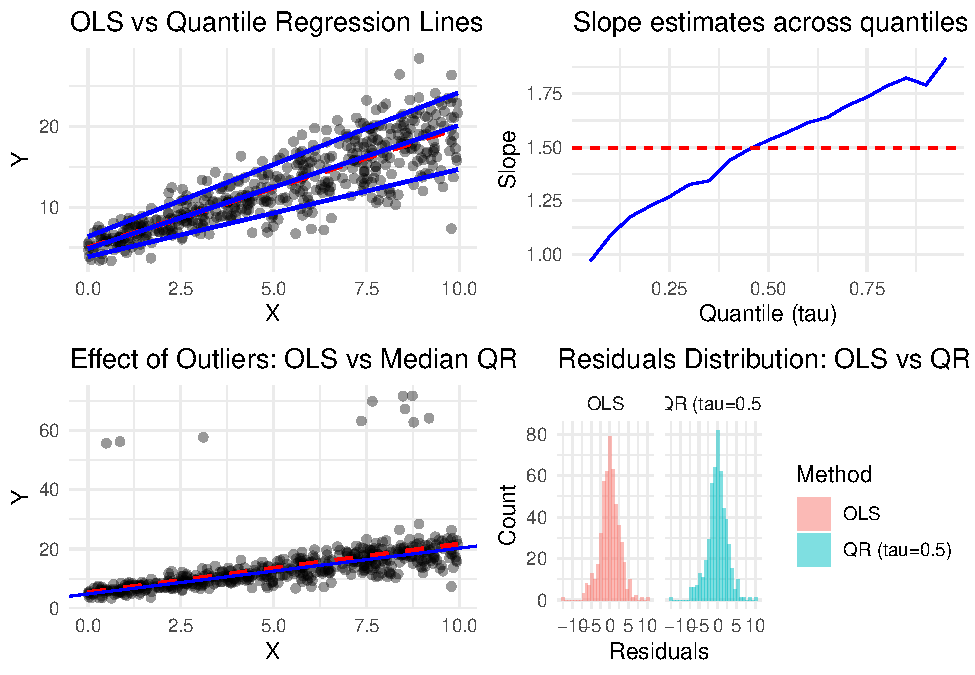
\includegraphics[width=0.8\linewidth]{ADR_project_files/figure-latex/other-plots-1} \end{center}

\section{Discussion \& Conclusions.}\label{discussion-conclusions.}

xxxxx

\textbf{\emph{Extras and considerations}}: This report has been made with a template in R Markdown, following the guidelines from \citep{Marcon2025}, and the most famous resource for the creation of reports in R Markdown, the bookdown package \citep{Xie2016}.

%----------------------------------------------------------------------------------------
%	REFERENCE LIST
%----------------------------------------------------------------------------------------

\bibliographystyle{apalike}
\makeatletter
% The filename has .bib extension that must be eliminated
\filename@parse{references.bib}
% parse stores the file name in base. Extension starts at the first dot, so don't use dots in file names.
\bibliography{\filename@base}
\makeatother


%----------------------------------------------------------------------------------------

\end{document}
